\documentclass[aspectratio=169,10pt]{beamer}

% fallback search path for ../theme/ when TEXINPUTS is not set (e.g. texmaker
% quick build); the makefile's TEXINPUTS takes precedence, so no conflict
\makeatletter
\providecommand*{\input@path}{}
\edef\input@path{\input@path{../theme/}{../theme/moloch/}}
\makeatother

\usepackage{icl26}
\usepackage{verbatim,fancyvrb}
\usepackage{ifthen}
\usepackage{minted}
\usepackage[kw]{pseudo}
\usepackage[export]{adjustbox}
\usepackage[edges]{forest}

% pseudocode: grey slanted comments, and highlights tight around the text of a line
\newcommand{\algcomment}[1]{\textsl{\grey{#1}}}
\colorlet{algdefect}{icBlue!18}
\colorlet{algfas}{icAccent!18}
\newcommand{\hlline}[2]{{\setlength{\fboxsep}{1.5pt}\hspace{-\fboxsep}\colorbox{#1}{\strut #2}\hspace{-\fboxsep}}}
\newcommand{\hldefect}[1]{\hlline{algdefect}{#1}}
\newcommand{\hlfas}[1]{\hlline{algfas}{#1}}
% every pseudo environment sits on a light grey, faintly yellow, background
%\definecolor{algbg}{HTML}{EEEDE0}
\definecolor{algbg}{HTML}{F0F0E8}
\newsavebox{\algbgbox}
\pseudoset{begin-tabular={\begin{lrbox}{\algbgbox}\begin{tabular}{\pseudopreamble}},
           end-tabular={\end{tabular}\end{lrbox}{\setlength{\fboxsep}{3pt}\colorbox{algbg}{\usebox{\algbgbox}}}}}
\newsavebox{\algcodebox}  % so a column beside the pseudocode can match its height
\newcommand{\legendswatch}[1]{\textcolor{#1}{\rule[-1mm]{5mm}{4mm}}}

% minted highlightlines: full-width codegreen bands, except lines listed by
% \codepinkline get tight codepink boxes
\colorlet{codegreen}{green!15}
\colorlet{codepink}{red!15}
\makeatletter
\newcommand{\codepinkline}[1]{\@namedef{codepink@#1}{}}
\codepinkline{3}\codepinkline{15}\codepinkline{16}  % SPECIFIC LINES FROM copref.py below
\let\codehl@full\FancyVerbHighlightLineFirst  % Middle, Last, Single are copies of First
\newcommand{\codehl@pick}[1]{%
  \ifcsname codepink@\the\value{FancyVerbLine}\endcsname
    {\let\FancyVerbFormatText\codehl@fmt#1}%
  \else
    \codehl@natural{#1}{\let\strut\codehl@strut\codehl@full{#1}}%
  \fi}
% the color fills one full line height (\strut is too short in the code font),
% so highlights on consecutive lines touch, but each box reports the text's
% natural height and depth, so line spacing matches the unhighlighted code
\newcommand{\codehl@strut}{\rule[-.3\baselineskip]{0pt}{\baselineskip}}
\newsavebox{\codehl@text}
\newcommand{\codehl@natural}[2]{%  typeset #2 with the height and depth of #1
  \sbox{\codehl@text}{#1}%
  \@tempdima=\ht\codehl@text \@tempdimb=\dp\codehl@text
  \sbox{\codehl@text}{#2}%
  \ht\codehl@text=\@tempdima \dp\codehl@text=\@tempdimb
  \usebox{\codehl@text}}
% pink: pass leading (active) spaces through, then box the rest tightly
\newcommand{\codehl@fmt}[1]{\codehl@strip#1\codehl@end}
\def\codehl@box#1\codehl@end{%
  \kern-1pt\codehl@natural{#1}{\setlength{\fboxsep}{0pt}\colorbox{codepink}{%
    \kern1pt\codehl@strut#1\kern1pt}}\kern-1pt}
\begingroup\catcode`\ =\active%
\gdef\codehl@strip{\futurelet\codehl@next\codehl@strip@i}%
\gdef\codehl@strip@i{\ifx\codehl@next \expandafter\codehl@eat\else\expandafter\codehl@box\fi}%
\gdef\codehl@eat { \codehl@strip}%
\endgroup
\let\FancyVerbHighlightLineFirst\codehl@pick
\let\FancyVerbHighlightLineMiddle\codehl@pick
\let\FancyVerbHighlightLineLast\codehl@pick
\let\FancyVerbHighlightLineSingle\codehl@pick
\makeatother

\newtheorem{proposition}[theorem]{Proposition}

\newcommand{\bb}{\mathbf{b}}
\newcommand{\bs}{\mathbf{s}}
\newcommand{\bu}{\mathbf{u}}

\newcommand{\bF}{\mathbf{F}}
\newcommand{\bG}{\mathbf{G}}

\newcommand{\blambda}{\symbf{\lambda}}
\newcommand{\bpsi}{\symbf{\psi}}
\newcommand{\bzero}{\symbf{0}}

\newcommand{\cA}{{\mathcal{A}}}
\newcommand{\cI}{{\mathcal{I}}}
\newcommand{\cT}{{\mathcal{T}}}
\newcommand{\cU}{{\mathcal{U}}}
\newcommand{\cD}{{\mathcal{D}}}

\newcommand{\RR}{{\mathbb{R}}}

\newcommand{\eps}{\epsilon}

\newcommand{\grad}{\nabla}
\newcommand{\Div}{\nabla\cdot}

\newcommand{\ip}[2]{\left\langle #1, #2 \right\rangle}

\newcommand{\lc}{{\text{\large $\circ$}}}

% grey comments on the right
\newcommand{\afcomm}[1]{\ensuremath{\text{\footnotesize \grey{$\leftarrow$ #1}}}}
\newcommand{\pcomm}[1]{\grey{\small (#1)}}
\newcommand{\pfcomm}[1]{\grey{\footnotesize (#1)}}
\newcommand{\efcomm}[1]{\grey{\footnotesize \emph{#1}}}

\newcommand{\blue}[1]{{\color{icBlue}#1}}

% author photos, from figs/people/, stacked at the far right of a frame:
%   \begin{withpeople}{\photo{a.jpg}{A.~Name} \photo{b.jpg}{B.~Name}} ... frame body ... \end{withpeople}
% (optional arg of \photo is the height, for longer stacks)
% use generic.png when none was found
\newcommand{\photo}[3][10mm]{\hbox to \linewidth{\hss\includegraphics[height=#1]{figs/people/#2}}\nointerlineskip\vskip0.2mm\hbox to \linewidth{\hss\tiny #3}\vskip0.6mm}
\newenvironment{withpeople}[1]
  {\def\peoplestack{#1}\begin{columns}[T,onlytextwidth]\begin{column}{0.88\textwidth}}
  {\end{column}\begin{column}{0.11\textwidth}\raggedleft\vspace*{-2mm}\peoplestack\end{column}\end{columns}}

% demo/figure not yet made
\newcommand{\placeholder}[3]{\fbox{\parbox[c][#2][c]{#1}{\centering \small \grey{PLACEHOLDER: #3}}}}



\title{New solvers for variational inequalities: a sample}
%\subtitle{Newton, \emph{a posteriori}, multilevel, and beyond}

\author{Ed Bueler}

\institute{University of Alaska Fairbanks}

\date{Imperial College London \, 2026}


\begin{document}

\begin{frame}
  \titlepage
\end{frame}

\begin{frame}[standout]
\begin{itemize}
\item I welcome questions at any time!
\item they are a \emph{good} use of time
\end{itemize}
\end{frame}


\begin{frame}{recall: definition of a variational inequality (VI)}

\begin{definition}
Given a \alert{Banach space $X$}, a closed and convex \alert{admissible subset $K\subset X$}, and \alert{$F: K\to X'$ continuous}, find $u\in K$ so that
  $$\boxed{\alert{\ip{F(u)}{v-u} \ge 0}} \qquad \text{for all } v\in K.$$
This is the \alert{variational inequality} for the data $K$ and $F$.
\end{definition}

\begin{itemize}
\item $K$ is generally given via inequalities (and/or equalities)
    \begin{itemize}
    \item[$\lc$] libraries may restrict to \alert{box constraints}, lower \& upper bounds on each dof
    \end{itemize}

\item $\ip{\cdot}{\cdot}$ denotes Hilbert space inner product, or dual pairing, according to context

\smallskip
\item this is a \alert{VI of the first kind} in some references
    \begin{itemize}
    \item[$\lc$] second kind: $\ip{F(u)}{v-u} + \Phi(v) - \Phi(u) \ge 0 \, \forall v$, for some semi-smooth $\Phi:K\to \RR$
    \end{itemize}
\end{itemize}
\end{frame}


\begin{frame}{recall: classical obstacle problem as a VI}

\begin{block}{classical obstacle problem}
for $X=H^1(\Omega)$, and an \alert{obstacle $\psi\in X$}, define the closed and convex admissible subset \alert{$K= \{v\in X : v\ge\psi \text{ and } v|_{\partial\Omega}=g\}$}, and seek $u\in K$ solving
    $$\alert{\int_\Omega \nabla u\cdot\nabla(v-u) \ge \int_\Omega f\,(v-u)} \quad \forall v\in K$$
\end{block}

\begin{columns}
\begin{column}{0.45\textwidth}
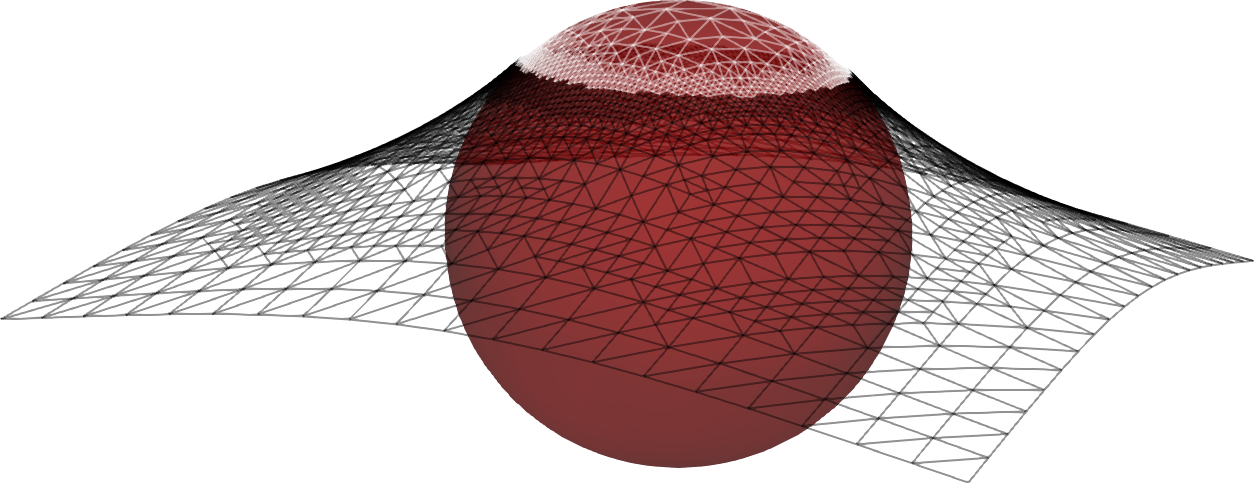
\includegraphics[width=0.8\textwidth]{figs/viamr-obstacle.png}

\hfill \begin{tikzpicture}[scale=0.4]
  \draw[line width=0.75pt] (-2.0,-2.0) -- (2.0,-2.0) -- (2.0,2.0) -- (-2.0,2.0) -- cycle;
  \node at (-1.3,1.3) {$E_u$};
  \draw[line width=1.0pt] (0.0,0.0) circle (0.69797);
  \node at (-0.1,-0.1) {$C_u$};
  \draw[-latex] (-2.3,-1.3) node[xshift=-3mm] {$\partial \Omega$} -- (-2.0,-1.3);
  \draw[-latex] (0.9,0.4) node[xshift=2mm] {$\Gamma_u$} -- (0.6,0.4);
  \draw[white] (2.0,1.0) -- (2.9,1.0);  % phantom helps balance figure
\end{tikzpicture}

\end{column}
\begin{column}{0.55\textwidth}
\begin{definition}
a solution $u$ defines subsets of $\Omega$:
\begin{align*}
&\text{\alert{inactive set} } & E_u &= \{x\,:\,u(x)>\psi(x)\} \\
&\text{\alert{active (contact) set} } & C_u &= \Omega \setminus E_u \\
&\text{\alert{free boundary} } & \Gamma_u &= \Omega\cap\partial E_u
\end{align*}
\end{definition}
\end{column}
\end{columns}
\end{frame}


\begin{frame}{recall: FE approximation, a finite-dimensional VI}

\begin{itemize}
\item assume \alert{$X_h=P_1$}, continuous \& piecewise-linear \hfill \pcomm{I'll return to Ciarlet's gauntlet at end}
\item define \alert{$\psi_h = I_h \psi$}, the nodal interpolant
\item define \alert{$K_h = \{v_h \in X_h : v_h \ge \psi_h \text{ and } v_h|_{\partial\Omega}=g\}$}
\item $K_h \subset X_h \subset X = H^1(\Omega)$, but generally \alert{$K_h \not\subset K$}

    \begin{itemize}
    \item[$\lc$] say ``conforming'' with care!
    \end{itemize}
\end{itemize}

\vspace{-10mm}
\hfill 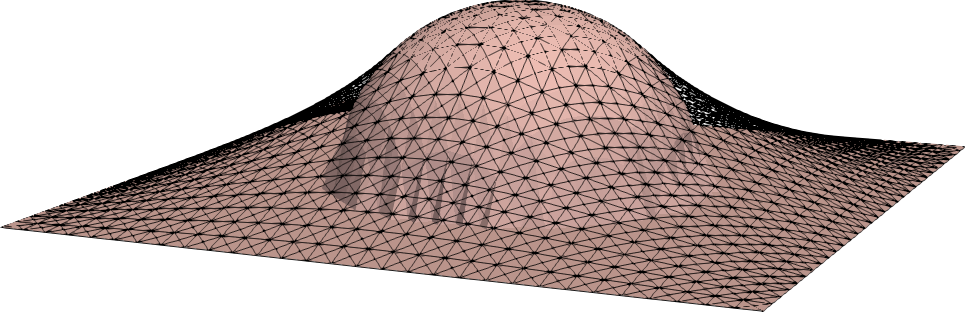
\includegraphics[width=0.6\textwidth]{figs/cop.png}

\medskip
\begin{block}{FE approximation of classical obstacle problem}
seek $u_h\in K_h$ so that \quad $\displaystyle \int_\Omega \grad u_h\cdot\grad(v_h-u_h) \ge \int_\Omega f\,(v_h-u_h) \quad \forall v_h\in K_h$
\end{block}
\end{frame}


\begin{frame}{outline}
  \tableofcontents
\end{frame}


\section{active-set Newton methods}


\begin{frame}[fragile]
\frametitle{active-set method demo: refine and count Newton iterations}

\begin{minipage}[t]{0.66\textwidth}
\only<1>{
\inputminted[fontsize=\fontsize{6}{7}\selectfont,highlightlines={20-23},highlightcolor=codegreen]{python}{code/copref.py}
}
\only<2>{
% see SPECIFIC LINES comment in preamble
\inputminted[fontsize=\fontsize{6}{7}\selectfont,highlightlines={3,15-16,20-23},highlightcolor=codegreen]{python}{code/coprefTrue.py}
}
\end{minipage}
\hfill
\begin{minipage}[t]{0.32\textwidth}
\vspace{-4.5mm}

% qrencode -o figs/qrcopref.png -s 10 -l L 'https://github.com/bueler/icl26/blob/main/talk2/code/copref.py'
% mogrify -trim -transparent white figs/qrcopref.png
\hspace{-15mm} \mbox{
\includegraphics[valign=t,width=0.25\textwidth]{figs/qrcopref.png} \qquad 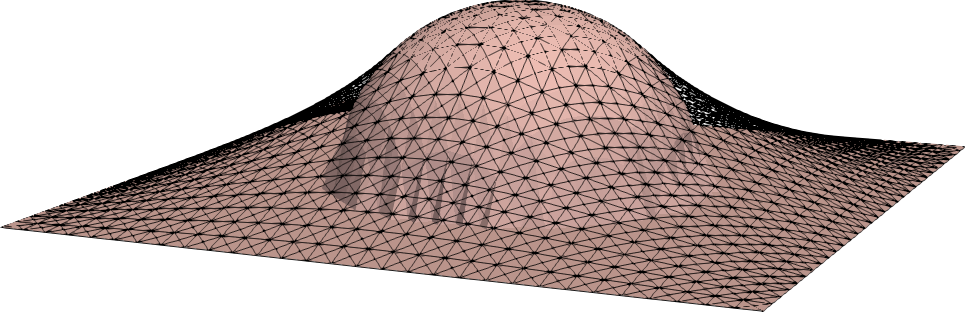
\includegraphics[valign=t,width=0.85\textwidth]{figs/cop.png}}

\bigskip
{\small
\begin{tabular}{rc}
mesh & Newton its. \\
\midrule
$10\times 10$   & 4 \\
$20\times 20$   & \only<1>{5}\only<2>{\alert{1}} \\
$40\times 40$   & \only<1>{8}\only<2>{\alert{2}} \\
$80\times 80$   & \only<1>{13}\only<2>{\alert{1}} \\
$160\times 160$ & \only<1>{24}\only<2>{\alert{2}} \\
$320\times 320$ & \only<1>{46}\only<2>{\alert{2}} 
\end{tabular}
}
\medskip
{\small
\begin{itemize}
\only<1>{
\item iterations \alert{double} at each refinement
}
\only<2>{
\item \strikeThrough{iterations double at each refinement}
}
\item<2> resolved by \alert{grid sequencing}
\end{itemize}
}
\end{minipage}
\end{frame}


\begin{frame}{language: \, residual $=$ multipliers $=$ dual variables}

\begin{itemize}
\item for $u_h\in X_h=P_1$, let \alert{$\bu=(u_i)\in\RR^N$} denote the nodal values

\smallskip
\item stiffness matrix $A$ and load vector $\bb$
\item the residual is \alert{$\bF(\bu) = A \bu - \bb \in \RR^N$}

    \begin{itemize}
    \item[$\lc$] in classical obstacle problem, the residual $\bF$ is a linear or affine map
    \end{itemize}
\smallskip
\item in optimization, $\alert{\lambda_i} = \bF(\bu)_i$ are the \alert{Lagrange multipliers} or \alert{dual variables}
\end{itemize}
\end{frame}


\begin{frame}{complementarity problem solvers}

\hfill 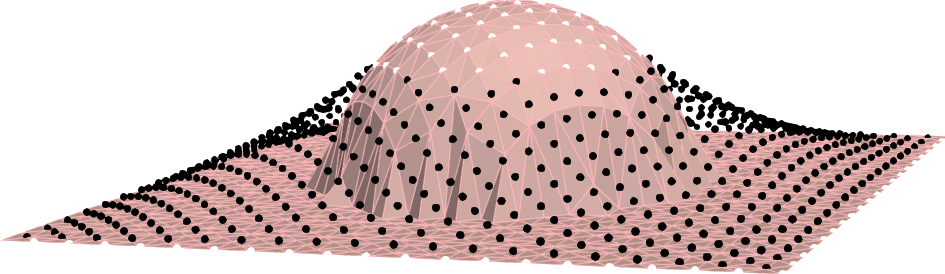
\includegraphics[width=0.4\textwidth]{figs/copactive.png}

\vspace{-5mm}
\begin{itemize}
\item $\lambda_i = \bF(\bu)_i$ are the Lagrange multipliers

\medskip
\begin{block}{complementarity problem (CP)}
for $i \in \{1,\dots,N\}$,
  $$u_i - \psi_i \ge 0, \qquad \lambda_i \ge 0, \qquad (u_i-\psi_i) \lambda_i = 0$$
\end{block}

\medskip
\item \alert{solving this CP} in $\RR^N$ is the goal in a FE VI problem
    \begin{itemize}
    \item[$\lc$] not \, ``$\lambda_i=0$'' or ``$\bF(\bu)=0$''
    \end{itemize}
\item at convergence, in exact arithmetic, generally $\blambda \ne 0$
    \begin{itemize}
    \item[$\lc$] \alert{$\lambda_i \ne 0 \implies u_i = \psi_i$ and $x_i\in C_{u_h}$} \hfill \pcomm{$x_i$ in active/contact set, white nodes}
    \end{itemize}

\smallskip
\item for bilateral bounds $\underline{\psi}_i \le u_i \le \overline{\psi}_i$ there is a straightforward CP generalization
\end{itemize}
\end{frame}


\begin{frame}[fragile]
\frametitle{active-set method: basic idea}

\begin{itemize}
\item \alert{VI problems are nonlinear}, even when the residual operator is linear or affine
    \begin{itemize}
    \item[$\lc$] we expect to iterate
    \end{itemize}
\item consider an admissible iterate $\bu^k \in \RR^N$, so that $u_i^k \ge \psi_i$
\item its \alert{active set} is the index set \quad \pcomm{white dots}
   $$\alert{\cA^k = \{i\,:\,u_i^k = \psi_i\}} \quad \subset \{1,\dots,N\} \hspace{30mm}$$

    \begin{itemize}
    \item[$\lc$] precisely, use tolerance: $\cA^k = \{i\,:\,u_i^k - \psi_i \le \operatorname{tol}\}$
    \item[$\lc$] inactive set is complement $\cI^k = \{1,\dots,N\}\setminus\cA^k$ \quad \pcomm{black dots}
    \end{itemize}

\vspace{-20mm}
\hfill 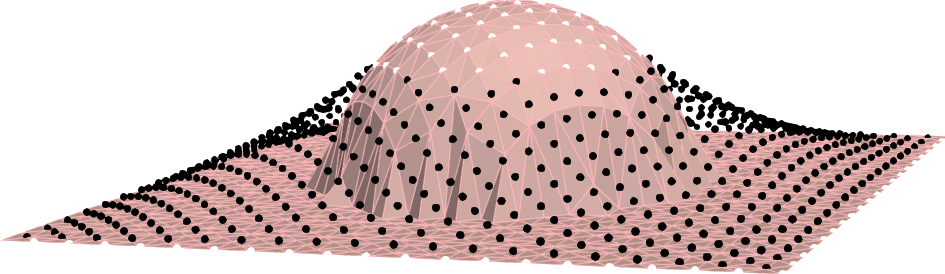
\includegraphics[width=0.3\textwidth]{figs/copactive.png}

\vspace{5mm}
\pause
\medskip
\item \alert{once one knows correct $\cA^k$, one solve determines correct $\bu=\bu^{k+1}$}
    \begin{itemize}
    \item[$\lc$] for classical obstacle problem: \quad $\bu_{\cA^k} = \bpsi_{\cA^k}, \quad (A\bu - \bb)_{\cI^k} = 0$
    \end{itemize}
\item of course, at $k=0$ we do not know the active set
\item what we see in practice \grey{$\to$}
\end{itemize}

\vspace{-7mm}
\hfill
\begin{minipage}{0.2\textwidth}
\begin{Verbatim}[fontsize=\tiny]
  0 SNES Function norm 3.624969175519e+00
  1 SNES Function norm 1.986779195391e+00
  2 SNES Function norm 6.109441485347e-01
  3 SNES Function norm 1.782534266924e-01
  4 SNES Function norm 4.555052324072e-02
  5 SNES Function norm 1.439049503152e-15
\end{Verbatim}
\end{minipage}
\hspace{20mm}
\end{frame}


\begin{frame}{the active-set method in PETSc}
\begin{withpeople}{\photo{generic.png}{S.~Benson} \photo{munson.jpg}{T.~Munson}}

\begin{itemize}
\item PETSc has SNES type \,\alert{\texttt{vinewtonrsls}} $=$ \texttt{rsls} \quad \pcomm{Benson \& Munson, 2006}
    \begin{itemize}
    \item[$\lc$] \texttt{rsls} = \underline{r}educed-\underline{s}pace with \underline{l}ine \underline{s}earch \quad \pcomm{reduced-space $=$ active-set}
    \end{itemize}
\item designed for nonlinear $\bF:\RR^N \to \RR^N$ and box constraints $\underline{\bpsi} \le \bu \le \overline{\bpsi}$
    \begin{itemize}
    \item[$\lc$] $\underline{\psi}_i = -\infty$ or $\overline{\psi}_i = +\infty$ permitted, so unconstrained dofs o.k.
    \item[$\lc$] \texttt{rsls} reduces to \texttt{newtonls} if no constraints are active
    \end{itemize}
\end{itemize}
\end{withpeople}

\begin{columns}
\begin{column}{0.5\textwidth}
\bigskip

{\footnotesize
\begin{pseudo}[label=, left-margin=0pt, topsep=0pt, line-height=1.25, indent-length=2.2em]
\texttt{rsls}$(\bpsi,\bu^0)$\texttt{:} \quad \tn{\efcomm{unilateral case}} \\+
$\bu^0 = \pi(\bu^0) = \max\{u_i^0, \psi_i\}$ \quad \tn{\efcomm{truncate}} \\
for $k=0,1,2,\dots$ \\+
  \alert{$\cA^k = \{i : u_i^k = \psi_i \tn{ and } F_i(u^k) > 0\}$} \tn{\&} $\cI^k = \big(\cA^k\big)^C$ \\
  $J_{\bF}(\bu^k)_{\cI^k,\cI^k}\, \bs_{\cI^k} = -\bF(\bu^k)_{\cI^k}$ \quad \tn{\efcomm{linear solve}} \\
  $\bs_{\cA^k} = 0$ \\
  $\bu^{k+1} = \pi(\bu^k+\alpha \bs)$ \quad \tn{\efcomm{truncated line search}} \\
  stop if \tn{(appropriate CP norm) $<\operatorname{tol}$} \\-
\end{pseudo}
}
\end{column}
\begin{column}{0.5\textwidth}
{\small
\begin{block}{RSLS = \texttt{vinewtonrsls}}
Newton step in inactive (reduced) space, with

line search over admissible states
\end{block}

\begin{itemize}
\item \alert{user's $\bF$ only sees admissible iterates}
\item linear solver is user's choice \pfcomm{CG, multigrid, \dots}
\item no parameter used in setting $\cA^k$
\end{itemize}
}
\end{column}
\end{columns}
\end{frame}


\begin{frame}{alternative view: semi-smooth Newton}

\begin{itemize}
\item complementarity is equivalent to a \alert{semi-smooth equation}:
    $$u_i\ge \psi_i, \,\, \lambda_i \ge 0, \,\, \lambda_i(u_i-\psi_i)=0 \quad \iff \quad \lambda_i - \max\{0,\lambda_i - \alert{c}\,(u_i-\psi_i)\} = 0$$

    \begin{itemize}
    \item[$\lc$] $\max\{0,x\}$ is semi-smooth, with a well-behaved directional derivative
    \item[$\lc$] equivalent for any $\alert{c}>0$
    \end{itemize}

\smallskip
\item idea: solve the VI by solving the \alert{primal-dual} nonlinear system $\bG(\bu,\blambda)=\bzero$:
    $$\bG(\bu,\blambda) = \begin{pmatrix} \bF(\bu) - \blambda \\ \blambda - \max\{\bzero,\blambda - \alert{c}(\bu-\bpsi)\} \end{pmatrix}$$
\item solve $\bG(\bu,\blambda)=\bzero$ using Newton's method, naturally
\end{itemize}
\end{frame}


\begin{frame}{primal-dual active-set is a Newton method}

\begin{itemize}
\item restrict to linear case $\bF(\bu) = A\bu - \bb$, with symmetric $A$ \, \pcomm{quadratic optimization; $\bF=\grad f$}
\end{itemize}

\medskip
\begin{columns}
\begin{column}{0.6\textwidth}
{\footnotesize
\begin{pseudo}[label=, left-margin=0pt, topsep=0pt, line-height=1.25, indent-length=2.2em]
\texttt{pdas}$(\bpsi,\bu^0,\alert{c})$\texttt{:} \quad \tn{\efcomm{unilateral case}} \\+
  $\cA^0=\emptyset$, $\cI^k=\{1,\dots,N\}$, $\blambda^0=\bzero$ \\
  for $k=0,1,2,\dots$ \\+
    $A_{\cI^k,\cI^k}\, \bs_{\cI^k} = \alert{-A_{\cI^k,\cA^k} (\bu^k - \bpsi)} -(A\bu^k-\bb)_{\cI^k}$ \quad \tn{\efcomm{linear solve}} \\
    $\bu_{\cI^k}^{k+1}=\bu_{\cI^k}^{k}+\bs_{\cI^k}$ \tn{\,\&\,} $\bu_{\cA^k}^{k+1}=\bpsi_{\cA^k}$ \\
    $\blambda^{k+1}_{\cA^k}=-(A\bu^{k+1}-\bb)_{\cA^k}$ \tn{\,\&\,} $\blambda^{k+1}_{\cI^k}=0$ \\
    \alert{$\cA^k = \{i : \lambda_i^k - c(u_i^k-\psi_i) > 0\}$} \tn{\,\&\,} $\cI^k = \big(\cA^k\big)^C$ \\
    stop if \tn{(appropriate CP norm) $<\operatorname{tol}$}
\end{pseudo}
}
\end{column}
\begin{column}{0.4\textwidth}
{\small
\begin{block}{PDAS = primal-dual active-set}
iterative quadratic optimization method which adjusts primal ($\bu$) and dual ($\blambda$) dofs via estimated active set
\end{block}

\begin{itemize}
\item note \alert{$c$} is used in setting $\cA^k$
\end{itemize}
}
\end{column}
\end{columns}

\begin{withpeople}{\photo{hintermueller.jpg}{M.~Hinterm\"uller} \photo[9mm]{generic.png}{K.~Ito} \photo{kunisch.jpg}{K.~Kunisch}}

\bigskip
\begin{theorem}[Hinterm\"uller, Ito \& Kunisch 2002]
\begin{itemize}
\item PDAS $=$ (semismooth Newton).  Thus converges locally superlinearly.
\item If $A$ is M-matrix then converges globally, and iterates $k>1$ are admissible.
\end{itemize}
\end{theorem}
\end{withpeople}
\end{frame}


\begin{frame}{recent clarity}

\begin{itemize}
\item in demo, RSLS iterations grew fast (w/o grid-sequencing)
\item what's going on?
\item for the quadratic optimization case,

{\alert{recent results provide clarity}}
\end{itemize}

\vspace{-20mm}
\hfill 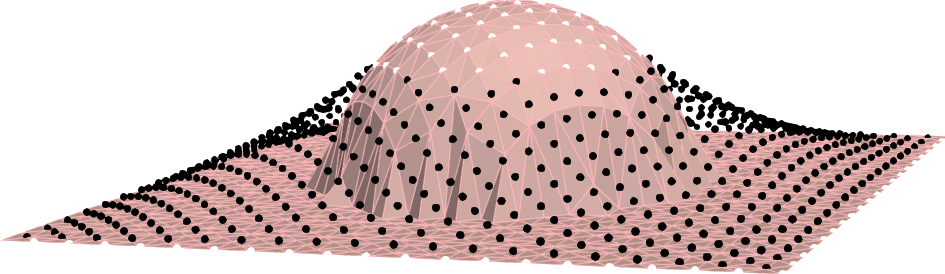
\includegraphics[width=0.4\textwidth]{figs/copactive.png}

\vspace{4mm}
\begin{withpeople}{\photo{papadopoulos.jpg}{I.~Papadopoulos} \photo{farrell.jpg}{P.~Farrell} \photo{surowiec.jpg}{T.~Surowiec} \photo{hintermueller.jpg}{M.~Hinterm\"uller}}

\vspace{-4mm}
\begin{theorem}[Papadopoulos, Farrell, \& Surowiec 2021, App.~A]
PETSc's RSLS is same as PDAS, but a half-step out of sync.
\end{theorem}

\begin{theorem}[``peeling'' theorem; Papadopoulos \& Hinterm\"uller 2026]
In PDAS, if $i\in\cA^k$, and its neighbors are in $\cA^k$, then $i\in\cA^{k+1}$.  \alert{A node can only de-activate if has an inactive set neighbor.}
\end{theorem}

\begin{itemize}
\item thus obstacle problem iterations (generically) grow exponentially
\item but Signorini problem iterations only grow mildly
\end{itemize}
\end{withpeople}
\end{frame}


\AtBeginSection[]
{
  \begin{frame}{outline}
  \tableofcontents[currentsection]
  \end{frame}
}

\section{multilevel solvers}


\begin{frame}{recall: grid-sequencing can fix mesh-dependent iterations}

\hfill%
{\footnotesize
\begin{tabular}{rcc}
mesh & \quad without \quad & w grid seq \\
\midrule
$10\times 10$   & 4  & 4 \\
$20\times 20$   & 5  & 1 \\
$40\times 40$   & 8  & 2 \\
$80\times 80$   & 13 & 1 \\
$160\times 160$ & 24 & 2 \\
$320\times 320$ & 46 & 2
\end{tabular}
}

\vspace{-18mm}
\begin{itemize}
\item iterations in the Firedrake demo \, \grey{$\to$}
    \begin{itemize}
    \item[$\lc$] for the classical obstacle problem
    \end{itemize}
\item from PETSc's RSLS, an active-set Newton solver

\vspace{10mm}
\item Newton iterations \alert{grow fast} with refinement, but this is fixed by \alert{grid sequencing}:
    \begin{itemize}
    \item[$\lc$] build \texttt{MeshHierarchy()}
    \item[$\lc$] prolong a coarse solution to the next-finer grid, as initial iterate
    \end{itemize}
\item grid-sequencing is a precursor to \alert{multigrid}
\end{itemize}
\end{frame}


\begin{frame}{notation for nonlinear weak form problems}

\begin{itemize}
\item consider solving general VI in which $F:X \to X'$ is \alert{nonlinear}

\smallskip
\begin{definitions}
Given a Banach space $X$ and $F: X\to X'$ smooth.

\smallskip
\alert{PDE($F$)}: \,  Find $u\in X$ s.t.~\,$\ip{F(u)}{v}=0 \, \forall v\in X$.

\smallskip
\alert{VI($K$,$F$)}: \, For $K\subset X$ closed \& convex, find $u\in K$ s.t.~\,$\alert{\ip{F(u)}{v-u} \ge 0} \, \forall v\in K$.
\end{definitions}

\item note PDE($F$) $=$ VI($X$,$F$)
\item functions \alert{$F: K\to X'$}, only defined on admissible inputs, are permitted in VI($K$,$F$)

\smallskip
\item well-posedness, regularity are nontrivial \dots \, next slides aspirational in general cases
\end{itemize}
\end{frame}


\begin{frame}{goal: optimal solvers for VIs}

\begin{itemize}
\item for PDE($F$) and VI($K$,$F$) there is a clear efficiency goal for FE solvers:

\begin{definition}
For a family of discrete problems $\{P_N\}$, a solver is \alert{optimal} if $O(N)$ arithmetic (or time) suffices to solve $P_N$, as $N\to\infty$.
\end{definition}

    \begin{itemize}
    \item[$\lc$] ``solve'' means to discretization accuracy
    \end{itemize}

\item \alert{constant in $O(N)$ definitely matters}
\item this definition only makes sense for fixed element degree \pcomm{$P_1$ in examples}
    \begin{itemize}
    \item[$\lc$] spectral and $hp$-FE ``use dofs better'' under $p$-refinement
    \end{itemize}
\item but this is a sensible \alert{goal}
\end{itemize}
\end{frame}


\begin{frame}{what's possible for PDE($F$)?}

\begin{itemize}
\item geometric multigrid can be an optimal PDE($F$) solver
    \begin{itemize}
    \item[$\lc$] assumes a well-behaved nonlinear elliptic $F$
    \end{itemize}
\item here is the \alert{Newton-multigrid} strategy
\end{itemize}

\bigskip

\begin{columns}
\begin{column}{0.35\textwidth}
\centering

\vspace{14mm}
\begin{tikzpicture}[scale=0.4]
  \pgfmathsetmacro\hstep{0.5}
  \pgfmathsetmacro\vstep{0.75}
  \pgfmathsetmacro\ceps{0.08}   % size of square for coarse grid

% V-cycle to finest (level 3)
  \pgfmathsetmacro\hoff{12*\hstep}
  \draw[shift={(\hoff,0)},black,thin] (0.0,3*\vstep) -- (\hstep,2*\vstep) --  (2*\hstep,\vstep) -- (3*\hstep,0.0) -- (4*\hstep,\vstep) -- (5*\hstep,2*\vstep) -- (6*\hstep,3*\vstep);
  \filldraw[shift={(\hoff,0)}] (0.0,3*\vstep) circle (2.5pt);
  \filldraw[shift={(\hoff,0)}] (\hstep,2*\vstep) circle (2.5pt);
  \filldraw[shift={(\hoff,0)}] (2*\hstep,\vstep) circle (2.5pt);
  \draw[shift={(\hoff,0)}]     (3*\hstep-\ceps,-\ceps) rectangle (3*\hstep+\ceps,+\ceps);
  \draw[shift={(\hoff,0)}]     (4*\hstep,\vstep) circle (2.5pt);
  \draw[shift={(\hoff,0)}]     (5*\hstep,2*\vstep) circle (2.5pt);
  \draw[shift={(\hoff,0)}]     (6*\hstep,3*\vstep) circle (2.5pt);

  \draw[white] (0, -\vstep) circle (2.5pt);
\end{tikzpicture}


\onslide<2>{\begin{tikzpicture}[scale=0.4]
  \pgfmathsetmacro\hstep{0.5}
  \pgfmathsetmacro\vstep{0.75}
  \pgfmathsetmacro\ceps{0.08}   % size of square for coarse grid

% solve coarsest and to level 1
  \pgfmathsetmacro\hoff{0*\hstep}
  \draw[shift={(\hoff,0)}]     (3*\hstep-\ceps,-\ceps) rectangle (3*\hstep+\ceps,+\ceps);
  \draw[shift={(\hoff,0)},black,thick] (3*\hstep,0.0) -- (4*\hstep,\vstep);

% V-cycle to level 1
  \pgfmathsetmacro\hoff{4*\hstep}
  \draw[shift={(\hoff,0)},black,thin] (0.0,\vstep) -- (\hstep,0.0) -- (2*\hstep,\vstep);
  \draw[shift={(\hoff,0)},black,thick] (2*\hstep,\vstep) -- (3*\hstep,2*\vstep);
  \filldraw[shift={(\hoff,0)}] (0.0,\vstep) circle (2.5pt);
  \draw[shift={(\hoff,0)}]     (\hstep-\ceps,-\ceps) rectangle (\hstep+\ceps,+\ceps);
  \draw[shift={(\hoff,0)}]     (2*\hstep,\vstep) circle (2.5pt);

% V-cycle to level 2
  \pgfmathsetmacro\hoff{7*\hstep}
  \draw[shift={(\hoff,0)},black,thin] (0.0,2*\vstep) --  (\hstep,\vstep) -- (2*\hstep,0.0) -- (3*\hstep,\vstep) -- (4*\hstep,2*\vstep);
  \draw[shift={(\hoff,0)},black,thick] (4*\hstep,2*\vstep) -- (5*\hstep,3*\vstep);
  \filldraw[shift={(\hoff,0)}] (0.0,2*\vstep) circle (2.5pt);
  \filldraw[shift={(\hoff,0)}] (\hstep,\vstep) circle (2.5pt);
  \draw[shift={(\hoff,0)}]     (2*\hstep-\ceps,-\ceps) rectangle (2*\hstep+\ceps,+\ceps);
  \draw[shift={(\hoff,0)}]     (3*\hstep,\vstep) circle (2.5pt);
  \draw[shift={(\hoff,0)}]     (4*\hstep,2*\vstep) circle (2.5pt);

% V-cycle to finest (level 3)
  \pgfmathsetmacro\hoff{12*\hstep}
  \draw[shift={(\hoff,0)},black,thin] (0.0,3*\vstep) -- (\hstep,2*\vstep) --  (2*\hstep,\vstep) -- (3*\hstep,0.0) -- (4*\hstep,\vstep) -- (5*\hstep,2*\vstep) -- (6*\hstep,3*\vstep);
  \filldraw[shift={(\hoff,0)}] (0.0,3*\vstep) circle (2.5pt);
  \filldraw[shift={(\hoff,0)}] (\hstep,2*\vstep) circle (2.5pt);
  \filldraw[shift={(\hoff,0)}] (2*\hstep,\vstep) circle (2.5pt);
  \draw[shift={(\hoff,0)}]     (3*\hstep-\ceps,-\ceps) rectangle (3*\hstep+\ceps,+\ceps);
  \draw[shift={(\hoff,0)}]     (4*\hstep,\vstep) circle (2.5pt);
  \draw[shift={(\hoff,0)}]     (5*\hstep,2*\vstep) circle (2.5pt);
  \draw[shift={(\hoff,0)}]     (6*\hstep,3*\vstep) circle (2.5pt);

  \draw[white] (0, -\vstep) circle (2.5pt);
\end{tikzpicture}

}
\end{column}
\begin{column}{0.65\textwidth}
\begin{tabular}{lll}
solver & optimal \\
\midrule
% solver tree for "what's possible" table; needs \usepackage[edges]{forest}
\begin{forest}
  begin draw/.code={\begin{tikzpicture}[baseline=(r.base)]}, for root={name=r},
  for tree={draw, font=\scriptsize, inner xsep=2pt, inner ysep=1.5pt, text height=1.5ex, text depth=0.4ex,
    edge={thin}, grow'=0, anchor=west, child anchor=west, calign=first, l sep=1.5mm, s sep=1.5mm,
    edge path'={([xshift=-4pt]!u.south east) |- (.child anchor)},
    after packing node={for children={s-=3.6mm}}}
  [Newton {\grey{$\times\ell$}} [LU]]
\end{forest}
 & no \\
% solver tree for "what's possible" table; needs \usepackage[edges]{forest}
\begin{forest}
  begin draw/.code={\begin{tikzpicture}[baseline=(r.base)]}, for root={name=r},
  for tree={draw, font=\scriptsize, inner xsep=2pt, inner ysep=1.5pt, text height=1.5ex, text depth=0.4ex,
    edge={thin}, grow'=0, anchor=west, child anchor=west, calign=first, l sep=1.5mm, s sep=1.5mm,
    edge path'={([xshift=-4pt]!u.south east) |- (.child anchor)},
    after packing node={for children={s-=3.6mm}}}
  [Newton [GMRES [mg V-cycle]]]
\end{forest}
 & \only<1>{yes \phantom{$O(N\log N)$}}\only<2>{\strikeThrough{yes} \grey{$O(N\log N)$}} \\
\onslide<2>{
% solver tree for "what's possible" table; needs \usepackage[edges]{forest}
\begin{forest}
  begin draw/.code={\begin{tikzpicture}[baseline=(r.base)]}, for root={name=r},
  for tree={draw, font=\scriptsize, inner xsep=2pt, inner ysep=1.5pt, text height=1.5ex, text depth=0.4ex,
    edge={thin}, grow'=0, anchor=west, child anchor=west, calign=first, l sep=1.5mm, s sep=1.5mm,
    edge path'={([xshift=-4pt]!u.south east) |- (.child anchor)},
    after packing node={for children={s-=3.6mm}}}
  [grid seq [Newton [GMRES [V-cycle {\grey{$\times k$}}]]]]
\end{forest}
 & yes \grey{$O(N)$}
}
\end{tabular}
\end{column}
\end{columns}

\bigskip
\begin{itemize}
\item<2> outer grid-sequencing makes an \alert{FMG cycle}
\end{itemize}
\end{frame}


\begin{frame}{what's possible from Newton-multigrid for VI($K$,$F$)?}

\begin{itemize}
\item for VI($K$,$F$), solving linear Newton-step problems by V-cycles is \alert{not} enough
\item a Newton active-set method like RSLS apparently \alert{already needs grid-sequencing} to give \alert{miNi}{\scriptsize $^{\operatorname{TM}}$} = \underline{m}esh-\underline{i}ndependent \underline{N}ewton \underline{i}terations
    \begin{itemize}
    \item[$\lc$] miNi is necessary but not sufficient for optimality on final mesh
    \end{itemize}
\end{itemize}

\bigskip
\begin{columns}
\begin{column}{0.35\textwidth}
\centering

\vspace{15mm}
\begin{tikzpicture}[scale=0.4]
  \pgfmathsetmacro\hstep{0.5}
  \pgfmathsetmacro\vstep{0.75}
  \pgfmathsetmacro\ceps{0.08}   % size of square for coarse grid

% just up side
  \pgfmathsetmacro\hoff{12*\hstep}
  \draw[shift={(\hoff,0)},black,thick] (3*\hstep,0.0) -- (4*\hstep,\vstep) -- (5*\hstep,2*\vstep) -- (6*\hstep,3*\vstep);
  \draw[shift={(\hoff,0)}]     (3*\hstep-\ceps,-\ceps) rectangle (3*\hstep+\ceps,+\ceps);
  \filldraw[shift={(\hoff,0)}]     (4*\hstep,\vstep) circle (2.5pt);
  \filldraw[shift={(\hoff,0)}]     (5*\hstep,2*\vstep) circle (2.5pt);
  \filldraw[shift={(\hoff,0)}]     (6*\hstep,3*\vstep) circle (2.5pt);

  \draw[white] (0, -\vstep) circle (2.5pt);  % phantom: same bounding box as vcycle.tex
\end{tikzpicture}



\begin{tikzpicture}[scale=0.4]
  \pgfmathsetmacro\hstep{0.5}
  \pgfmathsetmacro\vstep{0.75}
  \pgfmathsetmacro\ceps{0.08}   % size of square for coarse grid

% V-cycle to finest (level 3)
  \pgfmathsetmacro\hoff{12*\hstep}
  \draw[shift={(\hoff,0)},black,thin] (0.0,3*\vstep) -- (\hstep,2*\vstep) --  (2*\hstep,\vstep) -- (3*\hstep,0.0) -- (4*\hstep,\vstep) -- (5*\hstep,2*\vstep) -- (6*\hstep,3*\vstep);
  \filldraw[shift={(\hoff,0)}] (0.0,3*\vstep) circle (2.5pt);
  \filldraw[shift={(\hoff,0)}] (\hstep,2*\vstep) circle (2.5pt);
  \filldraw[shift={(\hoff,0)}] (2*\hstep,\vstep) circle (2.5pt);
  \draw[shift={(\hoff,0)}]     (3*\hstep-\ceps,-\ceps) rectangle (3*\hstep+\ceps,+\ceps);
  \draw[shift={(\hoff,0)}]     (4*\hstep,\vstep) circle (2.5pt);
  \draw[shift={(\hoff,0)}]     (5*\hstep,2*\vstep) circle (2.5pt);
  \draw[shift={(\hoff,0)}]     (6*\hstep,3*\vstep) circle (2.5pt);

  \draw[white] (0, -\vstep) circle (2.5pt);
\end{tikzpicture}



\onslide<2->{
\begin{tikzpicture}[scale=0.4]
  \pgfmathsetmacro\hstep{0.5}
  \pgfmathsetmacro\vstep{0.75}
  \pgfmathsetmacro\ceps{0.08}   % size of square for coarse grid

% solve coarsest and to level 1
  \pgfmathsetmacro\hoff{0*\hstep}
  \draw[shift={(\hoff,0)}]     (3*\hstep-\ceps,-\ceps) rectangle (3*\hstep+\ceps,+\ceps);
  \draw[shift={(\hoff,0)},black,thick] (3*\hstep,0.0) -- (4*\hstep,\vstep);

% V-cycle to level 1
  \pgfmathsetmacro\hoff{4*\hstep}
  \draw[shift={(\hoff,0)},black,thin] (0.0,\vstep) -- (\hstep,0.0) -- (2*\hstep,\vstep);
  \draw[shift={(\hoff,0)},black,thick] (2*\hstep,\vstep) -- (3*\hstep,2*\vstep);
  \filldraw[shift={(\hoff,0)}] (0.0,\vstep) circle (2.5pt);
  \draw[shift={(\hoff,0)}]     (\hstep-\ceps,-\ceps) rectangle (\hstep+\ceps,+\ceps);
  \draw[shift={(\hoff,0)}]     (2*\hstep,\vstep) circle (2.5pt);

% V-cycle to level 2
  \pgfmathsetmacro\hoff{7*\hstep}
  \draw[shift={(\hoff,0)},black,thin] (0.0,2*\vstep) --  (\hstep,\vstep) -- (2*\hstep,0.0) -- (3*\hstep,\vstep) -- (4*\hstep,2*\vstep);
  \draw[shift={(\hoff,0)},black,thick] (4*\hstep,2*\vstep) -- (5*\hstep,3*\vstep);
  \filldraw[shift={(\hoff,0)}] (0.0,2*\vstep) circle (2.5pt);
  \filldraw[shift={(\hoff,0)}] (\hstep,\vstep) circle (2.5pt);
  \draw[shift={(\hoff,0)}]     (2*\hstep-\ceps,-\ceps) rectangle (2*\hstep+\ceps,+\ceps);
  \draw[shift={(\hoff,0)}]     (3*\hstep,\vstep) circle (2.5pt);
  \draw[shift={(\hoff,0)}]     (4*\hstep,2*\vstep) circle (2.5pt);

% V-cycle to finest (level 3)
  \pgfmathsetmacro\hoff{12*\hstep}
  \draw[shift={(\hoff,0)},black,thin] (0.0,3*\vstep) -- (\hstep,2*\vstep) --  (2*\hstep,\vstep) -- (3*\hstep,0.0) -- (4*\hstep,\vstep) -- (5*\hstep,2*\vstep) -- (6*\hstep,3*\vstep);
  \filldraw[shift={(\hoff,0)}] (0.0,3*\vstep) circle (2.5pt);
  \filldraw[shift={(\hoff,0)}] (\hstep,2*\vstep) circle (2.5pt);
  \filldraw[shift={(\hoff,0)}] (2*\hstep,\vstep) circle (2.5pt);
  \draw[shift={(\hoff,0)}]     (3*\hstep-\ceps,-\ceps) rectangle (3*\hstep+\ceps,+\ceps);
  \draw[shift={(\hoff,0)}]     (4*\hstep,\vstep) circle (2.5pt);
  \draw[shift={(\hoff,0)}]     (5*\hstep,2*\vstep) circle (2.5pt);
  \draw[shift={(\hoff,0)}]     (6*\hstep,3*\vstep) circle (2.5pt);

  \draw[white] (0, -\vstep) circle (2.5pt);
\end{tikzpicture}


}
\end{column}
\begin{column}{0.65\textwidth}
\begin{tabular}{lll}
solver & miNi & optimal \\
\midrule
% solver tree for "what's possible" table; needs \usepackage[edges]{forest}
\begin{forest}
  begin draw/.code={\begin{tikzpicture}[baseline=(r.base)]}, for root={name=r},
  for tree={draw, font=\scriptsize, inner xsep=2pt, inner ysep=1.5pt, text height=1.5ex, text depth=0.4ex,
    edge={thin}, grow'=0, anchor=west, child anchor=west, calign=first, l sep=1.5mm, s sep=1.5mm,
    edge path'={([xshift=-4pt]!u.south east) |- (.child anchor)},
    after packing node={for children={s-=3.6mm}}}
  [RSLS {\grey{$\times\ell$}} [LU]]
\end{forest}
 & no & no \\
% solver tree for "what's possible" table; needs \usepackage[edges]{forest}
\begin{forest}
  begin draw/.code={\begin{tikzpicture}[baseline=(r.base)]}, for root={name=r},
  for tree={draw, font=\scriptsize, inner xsep=2pt, inner ysep=1.5pt, text height=1.5ex, text depth=0.4ex,
    edge={thin}, grow'=0, anchor=west, child anchor=west, calign=first, l sep=1.5mm, s sep=1.5mm,
    edge path'={([xshift=-4pt]!u.south east) |- (.child anchor)},
    after packing node={for children={s-=3.6mm}}}
  [grid seq [RSLS {\grey{$\times\ell$}} [LU]]]
\end{forest}
 & yes & no \\
% solver tree for "what's possible" table; needs \usepackage[edges]{forest}
\begin{forest}
  begin draw/.code={\begin{tikzpicture}[baseline=(r.base)]}, for root={name=r},
  for tree={draw, font=\scriptsize, inner xsep=2pt, inner ysep=1.5pt, text height=1.5ex, text depth=0.4ex,
    edge={thin}, grow'=0, anchor=west, child anchor=west, calign=first, l sep=1.5mm, s sep=1.5mm,
    edge path'={([xshift=-4pt]!u.south east) |- (.child anchor)},
    after packing node={for children={s-=3.6mm}}}
  [RSLS [GMRES [mg V-cycle]]]
\end{forest}
 & \alert{no} & no \\
\onslide<2->{
% solver tree for "what's possible" table; needs \usepackage[edges]{forest}
\begin{forest}
  begin draw/.code={\begin{tikzpicture}[baseline=(r.base)]}, for root={name=r},
  for tree={draw, font=\scriptsize, inner xsep=2pt, inner ysep=1.5pt, text height=1.5ex, text depth=0.4ex,
    edge={thin}, grow'=0, anchor=west, child anchor=west, calign=first, l sep=1.5mm, s sep=1.5mm,
    edge path'={([xshift=-4pt]!u.south east) |- (.child anchor)},
    after packing node={for children={s-=3.6mm}}}
  [grid seq [RSLS [GMRES [V-cycle {\grey{$\times k$}}]]]]
\end{forest}
 & yes & \alert{yes?}
}
\end{tabular}
\end{column}
\end{columns}
\end{frame}


% POSSIBLE SLIDE HERE: qrcode for code/copnm.py, with minimal table of results; note need for patch because of MatCreateSubMatrix and caching issues; these do not apply to FASCD


\begin{frame}{different strategy}

FIXME perspective: we want a more effective V-cycle for VIs

FIXME just show FASCD structure, and one-row table

FIXME add grid-sequenced FASCD tree
\begin{itemize}
\item FIXME
\end{itemize}

\bigskip
\begin{columns}
\begin{column}{0.35\textwidth}
\centering

\begin{tikzpicture}[scale=0.4]
  \pgfmathsetmacro\hstep{0.5}
  \pgfmathsetmacro\vstep{0.75}
  \pgfmathsetmacro\ceps{0.08}   % size of square for coarse grid

% V-cycle to finest (level 3)
  \pgfmathsetmacro\hoff{12*\hstep}
  \draw[shift={(\hoff,0)},black,thin] (0.0,3*\vstep) -- (\hstep,2*\vstep) --  (2*\hstep,\vstep) -- (3*\hstep,0.0) -- (4*\hstep,\vstep) -- (5*\hstep,2*\vstep) -- (6*\hstep,3*\vstep);
  \filldraw[shift={(\hoff,0)}] (0.0,3*\vstep) circle (2.5pt);
  \filldraw[shift={(\hoff,0)}] (\hstep,2*\vstep) circle (2.5pt);
  \filldraw[shift={(\hoff,0)}] (2*\hstep,\vstep) circle (2.5pt);
  \draw[shift={(\hoff,0)}]     (3*\hstep-\ceps,-\ceps) rectangle (3*\hstep+\ceps,+\ceps);
  \draw[shift={(\hoff,0)}]     (4*\hstep,\vstep) circle (2.5pt);
  \draw[shift={(\hoff,0)}]     (5*\hstep,2*\vstep) circle (2.5pt);
  \draw[shift={(\hoff,0)}]     (6*\hstep,3*\vstep) circle (2.5pt);

  \draw[white] (0, -\vstep) circle (2.5pt);
\end{tikzpicture}



\onslide<2>{\begin{tikzpicture}[scale=0.4]
  \pgfmathsetmacro\hstep{0.5}
  \pgfmathsetmacro\vstep{0.75}
  \pgfmathsetmacro\ceps{0.08}   % size of square for coarse grid

% solve coarsest and to level 1
  \pgfmathsetmacro\hoff{0*\hstep}
  \draw[shift={(\hoff,0)}]     (3*\hstep-\ceps,-\ceps) rectangle (3*\hstep+\ceps,+\ceps);
  \draw[shift={(\hoff,0)},black,thick] (3*\hstep,0.0) -- (4*\hstep,\vstep);

% V-cycle to level 1
  \pgfmathsetmacro\hoff{4*\hstep}
  \draw[shift={(\hoff,0)},black,thin] (0.0,\vstep) -- (\hstep,0.0) -- (2*\hstep,\vstep);
  \draw[shift={(\hoff,0)},black,thick] (2*\hstep,\vstep) -- (3*\hstep,2*\vstep);
  \filldraw[shift={(\hoff,0)}] (0.0,\vstep) circle (2.5pt);
  \draw[shift={(\hoff,0)}]     (\hstep-\ceps,-\ceps) rectangle (\hstep+\ceps,+\ceps);
  \draw[shift={(\hoff,0)}]     (2*\hstep,\vstep) circle (2.5pt);

% V-cycle to level 2
  \pgfmathsetmacro\hoff{7*\hstep}
  \draw[shift={(\hoff,0)},black,thin] (0.0,2*\vstep) --  (\hstep,\vstep) -- (2*\hstep,0.0) -- (3*\hstep,\vstep) -- (4*\hstep,2*\vstep);
  \draw[shift={(\hoff,0)},black,thick] (4*\hstep,2*\vstep) -- (5*\hstep,3*\vstep);
  \filldraw[shift={(\hoff,0)}] (0.0,2*\vstep) circle (2.5pt);
  \filldraw[shift={(\hoff,0)}] (\hstep,\vstep) circle (2.5pt);
  \draw[shift={(\hoff,0)}]     (2*\hstep-\ceps,-\ceps) rectangle (2*\hstep+\ceps,+\ceps);
  \draw[shift={(\hoff,0)}]     (3*\hstep,\vstep) circle (2.5pt);
  \draw[shift={(\hoff,0)}]     (4*\hstep,2*\vstep) circle (2.5pt);

% V-cycle to finest (level 3)
  \pgfmathsetmacro\hoff{12*\hstep}
  \draw[shift={(\hoff,0)},black,thin] (0.0,3*\vstep) -- (\hstep,2*\vstep) --  (2*\hstep,\vstep) -- (3*\hstep,0.0) -- (4*\hstep,\vstep) -- (5*\hstep,2*\vstep) -- (6*\hstep,3*\vstep);
  \filldraw[shift={(\hoff,0)}] (0.0,3*\vstep) circle (2.5pt);
  \filldraw[shift={(\hoff,0)}] (\hstep,2*\vstep) circle (2.5pt);
  \filldraw[shift={(\hoff,0)}] (2*\hstep,\vstep) circle (2.5pt);
  \draw[shift={(\hoff,0)}]     (3*\hstep-\ceps,-\ceps) rectangle (3*\hstep+\ceps,+\ceps);
  \draw[shift={(\hoff,0)}]     (4*\hstep,\vstep) circle (2.5pt);
  \draw[shift={(\hoff,0)}]     (5*\hstep,2*\vstep) circle (2.5pt);
  \draw[shift={(\hoff,0)}]     (6*\hstep,3*\vstep) circle (2.5pt);

  \draw[white] (0, -\vstep) circle (2.5pt);
\end{tikzpicture}

}
\end{column}
\begin{column}{0.65\textwidth}
\begin{tabular}{lll}
solver & miNi & optimal \\
\midrule
% solver tree for "what's possible" table; needs \usepackage[edges]{forest}
\begin{forest}
  begin draw/.code={\begin{tikzpicture}[baseline=(r.base)]}, for root={name=r},
  for tree={draw, font=\scriptsize, inner xsep=2pt, inner ysep=1.5pt, text height=1.5ex, text depth=0.4ex,
    edge={thin}, grow'=0, anchor=west, child anchor=west, calign=first, l sep=1.5mm, s sep=1.5mm,
    edge path'={([xshift=-4pt]!u.south east) |- (.child anchor)},
    after packing node={for children={s-=3.6mm}}}
  [FASCD
    [{\grey{\textit{smoother:}} RSLS} [Jacobi]]
    [{\grey{\textit{coarsest:}} RSLS} [LU]]]
\end{forest}
 & no & no \\
\onslide<2>{
% solver tree for "what's possible" table; needs \usepackage[edges]{forest}
\begin{forest}
  begin draw/.code={\begin{tikzpicture}[baseline=(r.base)]}, for root={name=r},
  for tree={draw, font=\scriptsize, inner xsep=2pt, inner ysep=1.5pt, text height=1.5ex, text depth=0.4ex,
    edge={thin}, grow'=0, anchor=west, child anchor=west, calign=first, l sep=1.5mm, s sep=1.5mm,
    edge path'={([xshift=-4pt]!u.south east) |- (.child anchor)},
    after packing node={for children={s-=3.6mm}}}
  [FASCD
    [{\grey{\textit{smoother:}} RSLS} [Jacobi]]
    [{\grey{\textit{coarsest:}} RSLS} [LU]]]
\end{forest}
 & yes & yes
}
\end{tabular}
\end{column}
\end{columns}
\end{frame}


\begin{frame}{constraint decomposition and FAS}
\begin{withpeople}{\photo{abrandt.jpg}{A.~Brandt} \photo{tai.jpg}{X.-C.~Tai} \photo{farrell.jpg}{P.~Farrell}}

\begin{itemize}
\item full approximation scheme (FAS; Brandt 1977): multigrid for \emph{nonlinear} problems, without global linearization
\item constraint decomposition (Tai 2003): for a subspace decomposition $V = \sum_i V_i$, write
    $$K = \sum_i K_i, \qquad K_i \subset V_i$$
\item FASCD (Bueler \& Farrell 2024) combines them, using mesh levels:
    \begin{itemize}
    \item[$\lc$] \alert{defect constraint} $\chi^J = \psi^J - w^J$ for the fine-level iterate $w^J$
    \item[$\lc$] monotone restriction $\chi^{j-1} = R^\oplus \chi^j$ generates coarser constraints
    \item[$\lc$] down-smoothing in sets $\cD^j$, up-smoothing in larger sets $\cU^j$
    \item[$\lc$] smoother: a few reduced-space Newton steps on each level
    \end{itemize}
\end{itemize}

\vspace{-5mm}
\hfill 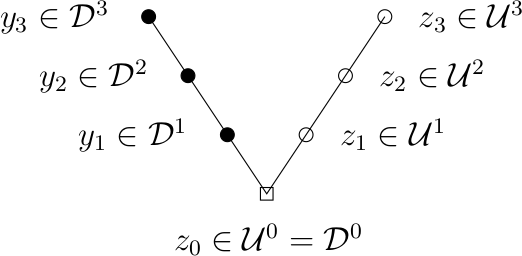
\includegraphics[width=0.35\textwidth]{figs/fascd-vcycle.png}
\end{withpeople}
\end{frame}


\begin{frame}{FASCD V-cycle}
\sbox{\algcodebox}{\begin{minipage}[t]{0.56\textwidth}
\vspace{0pt}
\footnotesize
\begin{pseudo}[label=, left-margin=0pt, topsep=0pt, idfont=\texttt, ctfont=\algcomment, ct-left=\quad\hfill, ct-right=, line-height=1.25, indent-length=2.2em,
               preamble={>{\pseudohpad}\pseudolabelalign>{\pseudosetup}w{l}{0.93\linewidth}<{\pseudohpad}}]
\texttt{fascd\_vcycle}$(J,\ell^J,\underline{\gamma}^J,\overline{\gamma}^J;w^J)$\texttt{:} \\+
  \hldefect{$\underline{\chi}^J, \, \overline{\chi}^J = \underline{\gamma}^J - w^J, \, \overline{\gamma}^J - w^J$} \\
  for $j=J$ downto $j=1$ \\+
    \hldefect{$\underline{\chi}^{j-1}, \, \overline{\chi}^{j-1} = R^\oplus \underline{\chi}^j, \, R^\ominus \overline{\chi}^j$} \\
    \hldefect{$\underline{\phi}^j, \, \overline{\phi}^j = \underline{\chi}^j - P\underline{\chi}^{j-1}, \, \overline{\chi}^j - P\overline{\chi}^{j-1}$} \\
    $y^j = 0$ \\
    $\text{\pr{smooth}}^{\text{\id{down}}}(\ell^j,\underline{\phi}^j,\overline{\phi}^j,w^j;y^j)$ \ct{VI problem in $\cD^j$} \\
    \hlfas{$w^{j-1} = R^\bullet(w^j + y^j)$} \\
    \hlfas{$\ell^{j-1} = f^{j-1}(w^{j-1}) + R \left(\ell^j - f^j(w^j+y^j)\right)$} \\-
  $z^0 = 0$ \\
  $\text{\pr{solve}}(\ell^0,\underline{\chi}^0,\overline{\chi}^0,w^0;z^0)$ \ct{VI problem in $\cU^0$} \\
  for $j=1$ to $j=J$ \\+
    \hlfas{$z^j = y^{j} + P z^{j-1}$} \\
    $\text{\pr{smooth}}^{\text{\id{up}}}(\ell^j,\underline{\chi}^j,\overline{\chi}^j,w^j;z^j)$ \ct{VI problem in $\cU^j$} \\-
  return $w^J+z^J$
\end{pseudo}
\end{minipage}}%
\usebox{\algcodebox}
\hfill % column on right
\begin{minipage}[t][\dimexpr\ht\algcodebox+\dp\algcodebox-2mm\relax][t]{0.4\textwidth}
\vspace{0pt}
{\small $\mitJ=3$ case:}

\bigskip
\hfill 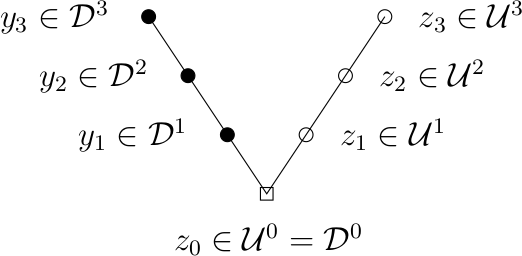
\includegraphics[width=0.85\textwidth]{figs/fascd-vcycle.png}

\vfill
\small
\mbox{\legendswatch{algdefect} \, construct defect constraints}

\bigskip
\mbox{\legendswatch{algfas} \, apply FAS formulas}
\end{minipage}
\end{frame}


\begin{frame}{FASCD results: classical obstacle problem}

\begin{itemize}
\item ball and spiral problems; up to $3.4\times 10^7$ nodes
\end{itemize}

{\small
\begin{center}
\begin{tabular}{rrcccccc}
     &       & \multicolumn{3}{c}{ball} & \multicolumn{3}{c}{spiral} \\
levels & nodes & RS only & V-cycles & FMG & RS only & V-cycles & FMG \\
\midrule
3  & 545              & 3  & 6  & +2 & 6  & 5  & +2 \\
5  & $8.3\times 10^3$ & 13 & 9  & +3 & 11 & 9  & +3 \\
7  & $1.3\times 10^5$ & 46 & 11 & +3 & 35 & 11 & +4 \\
9  & $2.1\times 10^6$ &    & 13 & +2 &    & 13 & +5 \\
11 & $3.4\times 10^7$ &    & 14 & +1 &    & 18 & +5 \\
\bottomrule
\end{tabular}
\end{center}
}

\begin{itemize}
\item RS only: iterations grow like resolution
\item V-cycles: slow growth; asymptotic rate about $0.1$
\item FMG: one full multigrid cycle, plus a few V-cycles
\end{itemize}

\vspace{-14mm}
\hfill 
\includegraphics[width=0.12\textwidth]{figs/ball-set.png} 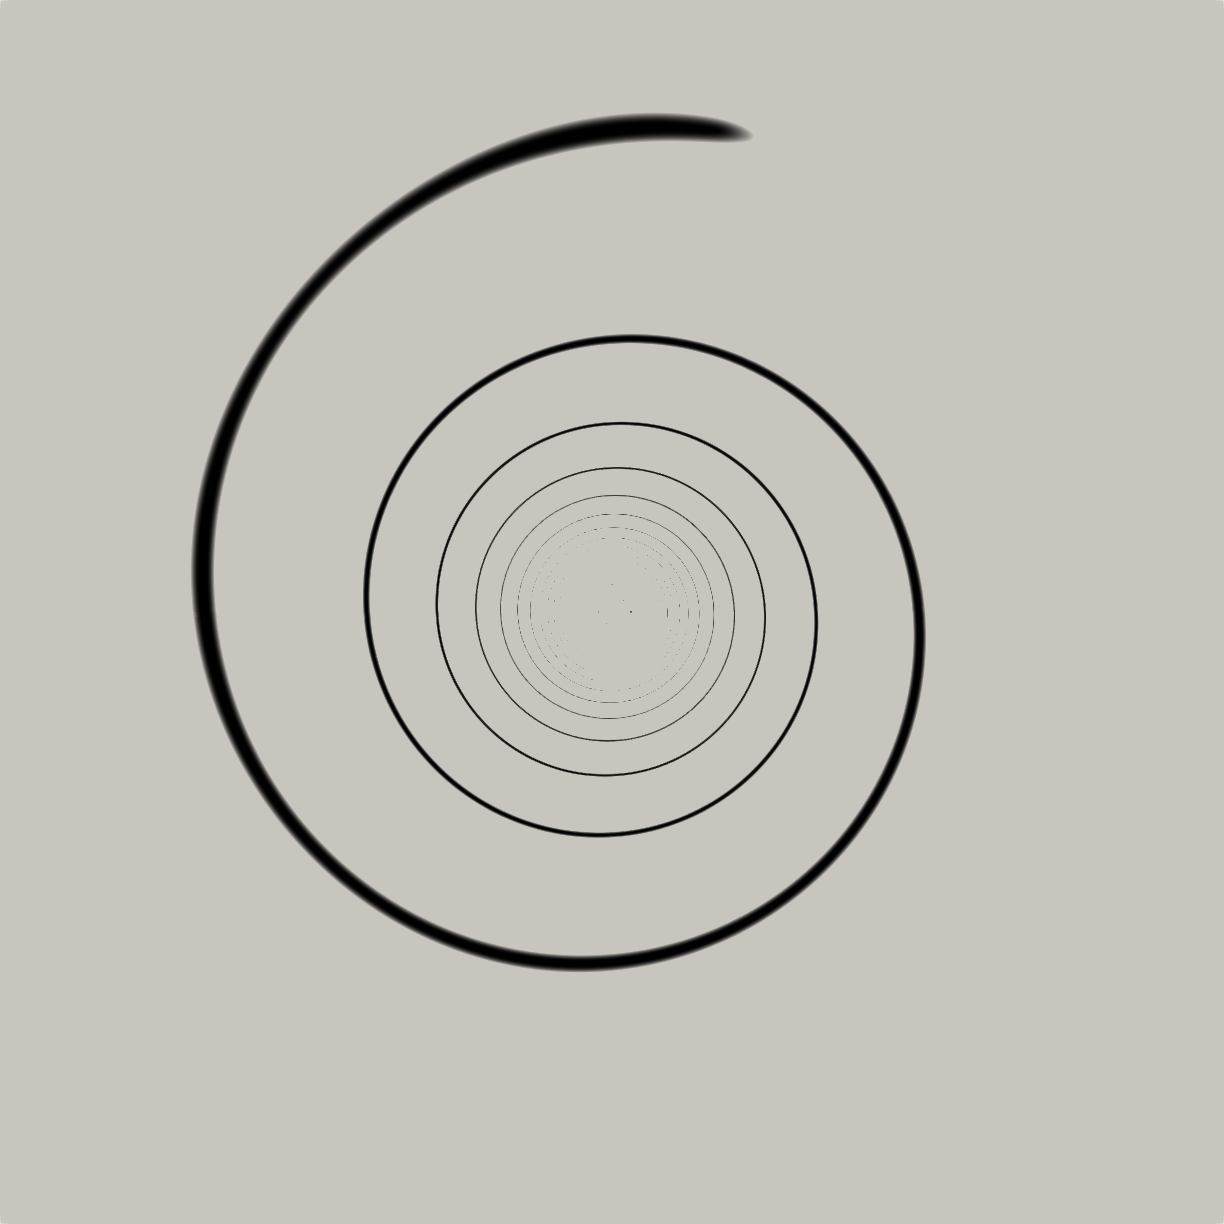
\includegraphics[width=0.12\textwidth]{figs/spiral-set.png}
\end{frame}


\begin{frame}{FASCD results: a glacier}

\begin{itemize}
\item shallow ice approximation: nonlinear, degenerate, and not an optimization
\item FMG with $Q_1$ elements; weak scaling on ARCHER2
\end{itemize}

\begin{center}
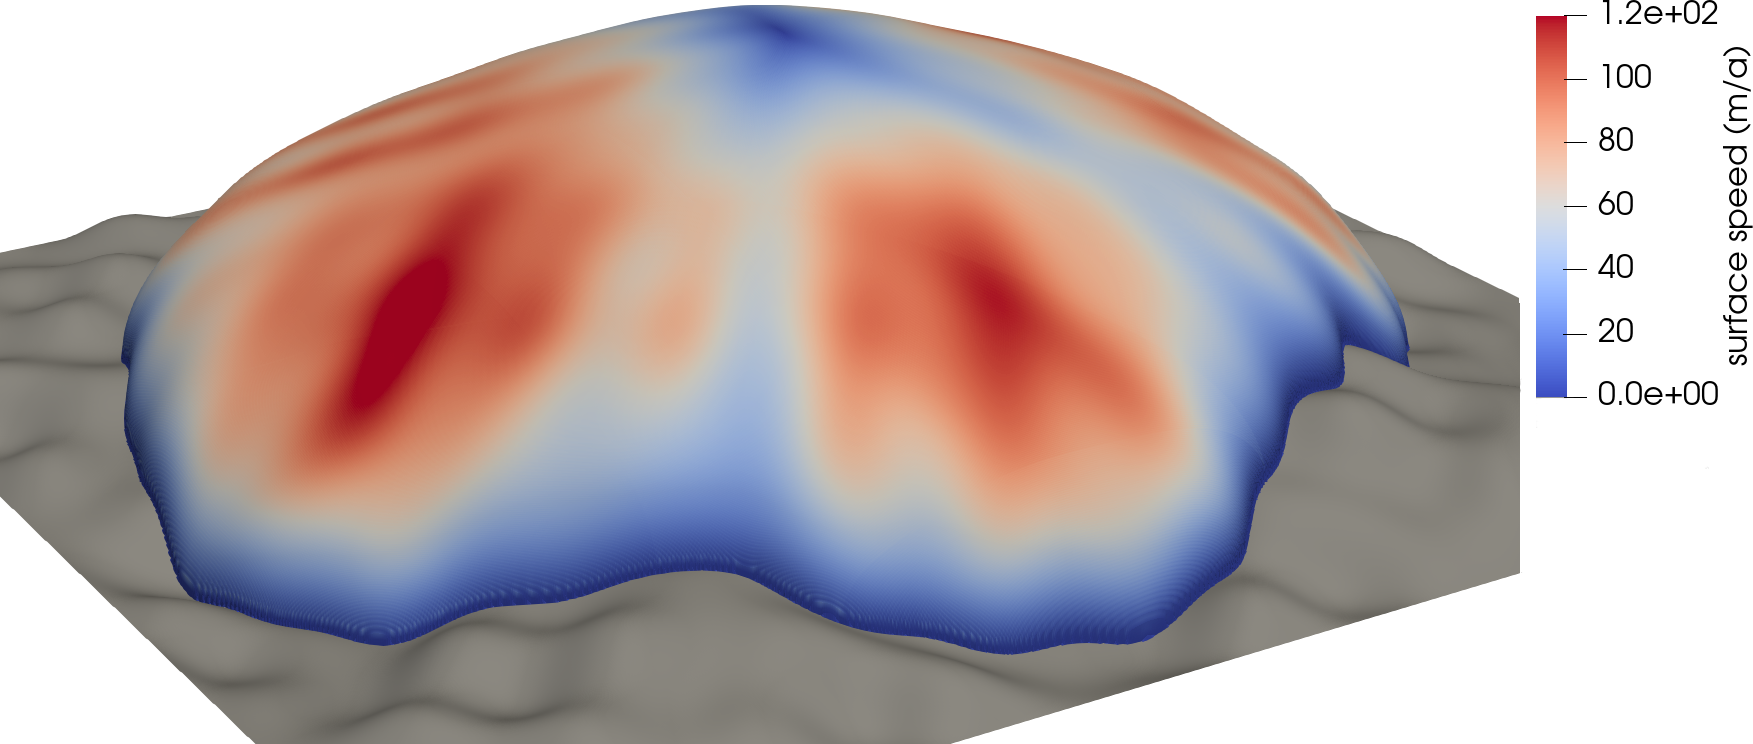
\includegraphics[width=0.55\textwidth]{figs/sialev8scene.png}
\end{center}

{\small
\begin{center}
\begin{tabular}{rrrcc}
processes & levels & nodes & V-cycles after FMG & time (s) \\
\midrule
1    & 6  & $641^2$   & +2 & 98 \\
16   & 8  & $2561^2$  & +2 & 124 \\
1024 & 11 & $20481^2$ & +1 & 177 \\
\bottomrule
\end{tabular}
\end{center}
}

\begin{itemize}
\item $4.1\times 10^8$ unknowns \pcomm{87.5 m resolution} in under 3 minutes
\end{itemize}
\end{frame}


\section[\emph{a posteriori} \& AMR]{\emph{a posteriori} estimates and adaptive refinement}

\begin{frame}{\emph{a posteriori} error estimates for PDEs}

\begin{itemize}
\item for the Poisson problem $-\grad^2 u = f$, the error $u-u_h$ is unknown, but the \alert{residual} of $u_h$ is computable
\item Babu\v{s}ka \& Rheinboldt (1978): on each element $T$,
    $$\eta_T^2 = h_T^2 \int_T |f + \grad^2 u_h|^2 + \frac{h_T}{2} \int_{\partial T} \left[\!\left[ \grad u_h\cdot n \right]\!\right]^2$$
\item then for $\eta^2 = \sum_T \eta_T^2$ there are constants so that
    $$c\,\eta \le |u-u_h|_{H^1} \le C\, \eta$$
    \begin{itemize}
    \item[$\lc$] upper bound: \alert{reliability}
    \item[$\lc$] lower bound: \alert{efficiency}
    \end{itemize}
\item adaptive mesh refinement (AMR) loop:
    $$\text{solve} \to \text{estimate} \to \text{mark} \to \text{refine} \to \text{solve} \to \dots$$
\end{itemize}
\end{frame}


\begin{frame}{what is different for VIs?}
\begin{withpeople}{\photo{generic.png}{A.~Veeser}}

\begin{itemize}
\item recall the residual $\sigma = F(u) - \ell$, e.g.~$\sigma = -\grad^2 u - f$
    \begin{itemize}
    \item[$\lc$] $\sigma \ge 0$ on the active set, and $\sigma = 0$ on the inactive set
    \item[$\lc$] $\sigma$ is the \alert{multiplier}; generally a measure
    \end{itemize}
\item the map from data $f$ to solution $u$ is not one-to-one:
    \begin{itemize}
    \item[$\lc$] changing $f$ inside the active set may not change $u$ at all
    \item[$\lc$] the information lost from $u$ is recorded in $\sigma$
    \end{itemize}
\end{itemize}

\begin{block}{Veeser's idea (2001)}
For VIs, estimate the error in the \alert{pair} $(u,\sigma)$, not just in $u$.
\end{block}

\begin{itemize}
\item Veeser (2001) proved reliable and efficient energy-norm estimators for $(u-u_h,\sigma-\sigma_h)$
\item the interior residual is localized to the (discrete) inactive set
\end{itemize}
\end{withpeople}
\end{frame}


\begin{frame}{pointwise \emph{a posteriori} bounds (NSV03)}
\begin{withpeople}{\photo{nochetto.jpg}{R.~Nochetto} \photo{siebert.jpg}{K.~Siebert} \photo{generic.png}{A.~Veeser}}

\begin{itemize}
\item Nochetto, Siebert \& Veeser (2003): maximum-norm bounds, with constraint imposed only at nodes
\end{itemize}

\begin{theorem}[NSV03]
For the $P_1$ classical obstacle problem there is a computable $E_h$ so that
    $$\max\left\{\|u-u_h\|_{L^\infty}, \,\, \|\sigma-\tilde\sigma_h\|_{W^{-2,\infty}}\right\} \le E_h,$$
and each term of $E_h$ is also locally efficient.
\end{theorem}

\vspace{-1mm}
{\small
\begin{align*}
E_h &= C_0 |\log h_{\min}|^2 \|h^2 R_\infty\|_\infty && \afcomm{residual, localized to inactive set} \\
    &\quad + C_1 |\log h_{\min}|^2 \|h^2 \grad\sigma_h\|_{d} && \afcomm{quadrature} \\
    &\quad + \|(\psi - u_h)^+\|_\infty + \|(u_h-\psi)^+\|_{\infty;\{\sigma_h>0\}} && \afcomm{obstacle approx.~and detachment} \\
    &\quad + \|g - I_h g\|_{\infty;\partial\Omega} && \afcomm{boundary data}
\end{align*}
}
\end{withpeople}
\end{frame}


\begin{frame}{VIAMR: AMR for the free boundary}
\begin{withpeople}{\photo{fochesatto.jpg}{S.~Fochesatto}}

\begin{itemize}
\item often the \alert{free boundary location} is the goal
\item VIAMR: a Firedrake-based library
\item separate two concerns, then recombine:
    \begin{itemize}
    \item[1.] \alert{UDO}: refine near the free boundary
    \item[2.] \alert{BR}: estimator in the inactive set
    \end{itemize}
\item UDO $=$ unstructured dilation operator:
    \begin{itemize}
    \item[$\lc$] mark elements with both active and inactive vertices
    \item[$\lc$] dilate the marking by $n$ layers of neighbors
    \end{itemize}
\item mark by the union, then refine
\end{itemize}

\vspace{-38mm}
\hfill 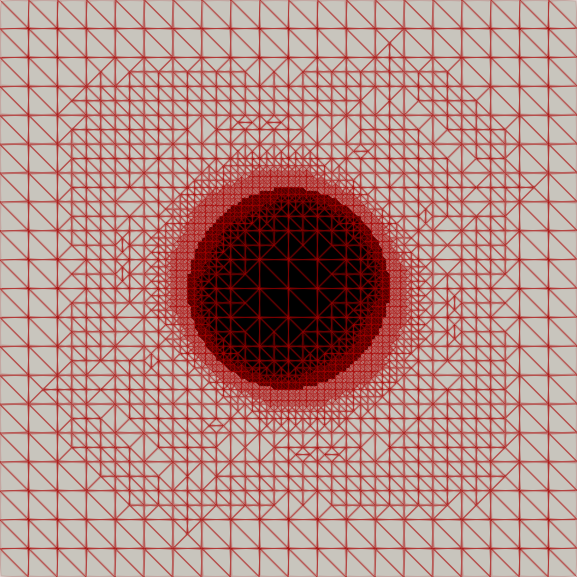
\includegraphics[width=0.24\textwidth]{figs/sphereudo.png}
\end{withpeople}
\end{frame}


\begin{frame}[fragile]
\frametitle{demo: VIAMR}

\begin{itemize}
\item after solving for $u_h$ \pcomm{as in \texttt{cop.py}}, refine by UDO+BR:
\end{itemize}

\begin{minted}[fontsize=\scriptsize]{python}
from viamr import VIAMR
amr = VIAMR()
fbmark = amr.udomark(uh, psih, n=1)                 # near free boundary
residual = -div(grad(uh))
imark, _, _ = amr.brinactivemark(uh, psih, residual, theta=0.7)  # in inactive set
mark = amr.unionmarks(fbmark, imark)
refinedmesh = amr.refinemarkedelements(mesh, mark)
\end{minted}

\medskip
\begin{itemize}
\item repeat: solve on the refined mesh, using the previous solution as initial iterate
\end{itemize}

\medskip
\placeholder{0.8\textwidth}{30mm}{live demo or figure: a few levels of UDO+BR refinement on the hemisphere obstacle}
\end{frame}


\begin{frame}{comparison: UDO+BR versus NSV03}

\begin{itemize}
\item FIXME NOT BILATERAL bilateral example again, both methods \hfill \grey{\small \texttt{viamr/examples/bilateral.py}}
\end{itemize}

\begin{center}
FIXME
\end{center}

\placeholder{0.8\textwidth}{12mm}{rerun at larger target; what is the take-away?}
\end{frame}


\section[higher-order \& latent-variable]{gloss: higher-order and latent-variable methods}

\begin{frame}{high-order bounds via the Bernstein basis}
\begin{withpeople}{\photo{kirby.jpg}{R.~Kirby} \photo{shapero.jpg}{D.~Shapero}}

\begin{itemize}
\item recall from last week: nodal values $\ge 0$ do not imply $v_h\ge 0$ for $P_k$, $k\ge 2$
\item Bernstein basis on $[0,1]$: \, $B_i^n(x) = \binom{n}{i} x^i (1-x)^{n-i}$
    \begin{itemize}
    \item[$\lc$] nonnegative partition of unity
    \item[$\lc$] $p = \sum_i p_i B_i^n$ lies in the convex hull of its coefficients (control net)
    \item[$\lc$] so \alert{coefficients $\ge 0$ implies $p\ge 0$} \pcomm{converse false}
    \item[$\lc$] extends to simplices via barycentric coordinates
    \end{itemize}
\item Kirby \& Shapero (2024): solve a VI over bounds-satisfying $P_k$
    \begin{itemize}
    \item[$\lc$] e.g.~$0\le u\le 1$ for advection-diffusion
    \item[$\lc$] C\'ea-type theorem; constrained $P_k$ approximates well
    \item[$\lc$] bounds on Bernstein coefficients: optimal orders observed
    \end{itemize}
\item but the \emph{continuum} problem is a PDE, not a VI
\end{itemize}
\end{withpeople}
\end{frame}


\begin{frame}{latent variable proximal point (LVPP)}
\begin{withpeople}{\photo{dokken.jpg}{J.~Dokken} \photo{farrell.jpg}{P.~Farrell} \photo{keith.jpg}{B.~Keith} \photo{papadopoulos.jpg}{I.~Papadopoulos} \photo{surowiec.jpg}{T.~Surowiec}}

\begin{itemize}
\item Dokken, Farrell, Keith, Papadopoulos \& Surowiec (2025)
\item Bregman proximal point iteration, using a \alert{latent} variable $\phi$:
    \, $u = \psi + e^{\phi} > \psi$
\item classical obstacle problem: given $\phi^{k-1}$, solve a nonlinear PDE system for $(u^k,\phi^k)$:
\begin{align*}
\alpha_k \int_\Omega \grad u^k\cdot\grad v + \int_\Omega \phi^k v &= \alpha_k \int_\Omega f v + \int_\Omega \phi^{k-1} v \\
\int_\Omega u^k w - \int_\Omega (\psi + e^{\phi^k})\, w &= 0
\end{align*}
\item no constraints to discretize: any FE spaces and degree, standard Newton
\item mesh-independent iterations observed; $\tilde u_h = \psi + e^{\phi_h}$ satisfies the bound
\item also contact, fracture, plasticity, Monge--Amp\`ere, \dots
\end{itemize}
\end{withpeople}
\end{frame}


\begin{frame}{summary}

\begin{itemize}
\item active-set Newton methods (PDAS, RS) are Newton methods, but iterations grow under refinement
    \begin{itemize}
    \item[$\lc$] the active set peels away one layer per iteration
    \end{itemize}
\item \emph{a posteriori} estimates for VIs control the pair $(u,\sigma)$
    \begin{itemize}
    \item[$\lc$] AMR should target the free boundary \emph{and} the PDE in the inactive set
    \end{itemize}
\item multilevel methods give mesh-independence:
    \begin{itemize}
    \item[$\lc$] grid sequencing $+$ Newton-multigrid, or FASCD
    \end{itemize}
\item new ideas: Bernstein bounds for high order, and LVPP
\end{itemize}

\pause
\centering
{\Large
\bigskip\bigskip
\alert{thank you for listening!}

\bigskip
\alert{questions?}
}
\end{frame}


\begin{frame}[allowframebreaks]{references}
%\begin{frame}{references}
% inputed at end of talk1.tex
% blue link text; local, since talk1.tex inputs this inside a frame
\let\plainhref\href
\renewcommand{\href}[2]{\plainhref{#1}{\textcolor{icBlue}{#2}}}

\setlength{\leftmargini}{1em}  % bullets near the left margin, not indented
\begin{itemize}\setlength{\itemsep}{2pt}
\footnotesize
@Article{BensonMunson2006,
  AUTHOR    = {S. Benson and T. Munson},
  TITLE     = {Flexible complementarity solvers for large-scale applications},
  JOURNAL   = {Optimization Methods and Software},
  VOLUME    = {21},
  NUMBER    = {1},
  PAGES     = {155--168},
  YEAR      = {2006},
}

\item E.~Bueler (2021). \href{https://doi.org/10.1137/1.9781611976311}{\emph{PETSc for Partial Differential Equations: Numerical Solutions in C and Python}}, SIAM Press

@misc{Bueler2026,
	author = {Ed Bueler},
	title = {Pointwise a posteriori error bounds for bilateral Laplacian obstacle problems},
	note = {in preparation},
	year = {2026},
}

@article{BuelerFarrell2024,
   author={Bueler, Ed and Farrell, Patrick E.},
   title={A full approximation scheme multilevel method for nonlinear variational inequalities},
   volume={46},
   number={4},
   journal={SIAM J. Sci. Comput.},
   year={2024},
   DOI={10.1137/23m1594200},
   pages={A2421--A2444},
}

@article{Dokkenetal2025,
  title={The latent variable proximal point algorithm for variational problems with inequality constraints},
  author={Dokken, J{\o}rgen S and Farrell, Patrick E and Keith, Brendan and Papadopoulos, Ioannis PA and Surowiec, Thomas M},
  journal={Computer Methods in Applied Mechanics and Engineering},
  volume={445},
  pages={118181},
  year={2025},
}

\item R.~Falk (1974).  \href{https://doi.org/10.1090/S0025-5718-1974-0391502-8}{\emph{Error estimates for the approximation of a class of variational inequalities}}, Math.~Comp.~28 (128), 963--971

@article{GraeserKornhuber2009,
	author = {Gr\"aser, Carsten and Kornhuber, Ralf},
	title = {Multigrid methods for obstacle problems},
	volume = {27},
	number = {1},
	journal = {Journal of Computational Mathematics},
	year = {2009},
	pages = {1--44},
}

@article{HintermullerItoKunisch2002primal,
    title={The primal-dual active set strategy as a semismooth Newton method},
    author={Hinterm{\"u}ller, Michael and Ito, Kazufumi and Kunisch, Karl},
    journal={SIAM Journal on Optimization},
    volume={13},
    number={3},
    pages={865--888},
    year={2002},
}

\item D.~Kinderlehrer \& G.~Stampacchia (1980). \href{https://doi.org/10.1137/1.9780898719451}{\emph{An Introduction to Variational Inequalities and their Applications}}, SIAM Classics 31

@article{KirbyShapero2024,
  title={High-order bounds-satisfying approximation of partial differential equations via finite element variational inequalities},
  author={Kirby, Robert C and Shapero, Daniel},
  journal={Numerische Mathematik},
  volume={156},
  number={3},
  pages={927--947},
  year={2024},
}

@article{NSV03,
    title={Pointwise a posteriori error control for elliptic obstacle problems},
    author={Nochetto, Ricardo H and Siebert, Kunibert G and Veeser, Andreas},
    journal={Numerische Mathematik},
    volume={95},
    number={1},
    pages={163--195},
    year={2003},
}

@misc{PapadopoulosHintermuller2026,
    title={Mesh-dependent iteration count growth in primal-dual active set strategies}, 
    author={Ioannis P. A. Papadopoulos and Michael Hintermüller},
    year={2026},
    eprint={2607.26622},
    archivePrefix={arXiv},
    url={https://arxiv.org/abs/2607.26622}, 
}
\end{itemize}

\end{frame}

\end{document}
